\documentclass[12pt]{article}
\usepackage{amsthm}
\usepackage[english]{babel}
\usepackage{graphicx}
\usepackage{epstopdf}
\usepackage{float}
\usepackage{subcaption}
\usepackage{url}
\title{\textbf{Style Transfer}}
\author{Ravinder Rai}
\date{\today}

\begin{document} 


\begin{titlepage}
\centering

\maketitle

\end{titlepage}

\newpage
\section{Definition}
\subsection{Project Overview}
In the subject of Machine Learning, there is an artistic problem called Style Transfer. Style Transfer lies in the field of deep neural networks and image classification, and while it is a relatively new problem, it has already seen a few notable solutions. One such solution is in Gatys' paper \cite{Neural}, in which this project will follow quite closely. Image classification is a popular problem in machine learning, where the goal is to detect specific objects in any given image, and it has many applications like face detection and even self-driving cars. The methodology of image classification is to use neural networks, which essentially have small image filters that try and detect import features in images, and associate them with an object of interest. A collection of these image filters can provide necessary texture information, which we can call the style of an image. In the past, capturing the style of an image was used to detect the time periods of other images (by seeing if they had a similar style), but here the idea of Style Transfer is to capture the style of some image, and recreate another image with that same style. This problem is mostly just a fun problem, which could be done by artists on their own, but the problem was that there was no real way to formulate or replicate Style Transfer results. However, with the help of image classification, interest in solving this problem with Machine Learning developed, and there are now replicable results.

\subsection{Problem Statement}
The problem in this project is to replicate Figure 2C in \cite{Neural} as closely as possible. The image Figure 2C in \cite{Neural} can be used as a guidance for how well my solution works, and is essentially the solution to the project. The project has been changed slightly from the original proposal, in that instead of simply replicating Figure 2C in \cite{Neural}, code has been taken from \cite{Github}, and the goal is now to replicate the image but in a timely manner, with a white-noise image (this change is due to the fact that run time takes too long, and will be explained in more detail later). There will also be a loss function by which accuracy can be measured. This loss function is a combination of both the style loss and content loss. Here, the content loss refers to the content image, which is the basis image that we are trying to recreate with a different style. The content loss is essentially a difference between the features on the original/content image and the  image that the neural network will create. Similarly, the style loss refers to the image whose style we are trying to capture. The style loss function will also be made up of a difference between the original style image and the image that the neural network creates. The total loss function will be a combination of both of these two style functions, and will be of the form:
\begin{equation}
Loss_{total} = \alpha * Loss_{content} + \beta * Loss_{style}
\end{equation}
$\alpha$ and $\beta$ will be tuned by trail and error to give the most optimal results. The ultimate solution will be to replicate figure 2C in \cite{Image}, while simultaneously minimizing the loss function such that the result is reproducible. Ultimately, this project boils down to finding the best optimizer, with its own optimal hyper-parameters.

\begin{figure}
\centering
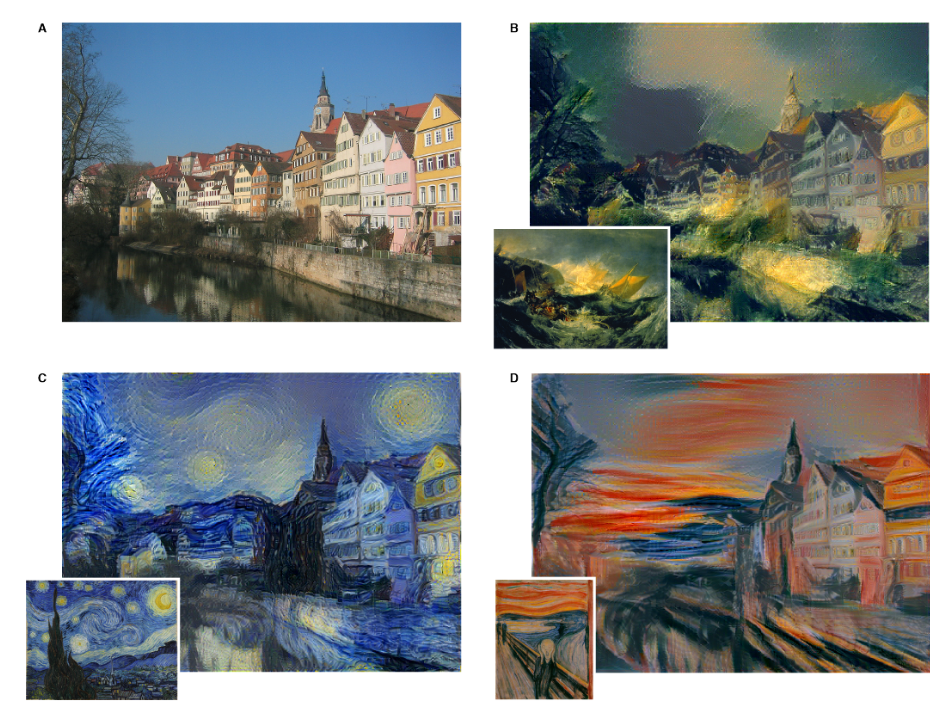
\includegraphics[totalheight=8cm]{Figure2.png}
    \caption{Figure 2 (A-D) used in \cite{Neural}. Image C is the solution image, with the image on the bottom left being the style image, and image A being the content image. Figure 2 in \cite{Neural} is identical to Figure 3 in \cite{Image}}
    \label{fig:solution}
\end{figure}

\subsection{Metrics}
The performance of the model can be measured by use of the total loss function ($Loss_{total}$) from above, and by the output image. If the output image is obviously not similar to the intended solution image in \cite{Neural, Image}, but the total loss function is minimal, then one would rate the model as a failing model. Similarly, if the output image is clearly similar to the solution image, but the total loss function outputs a large value, then one should rate the model as a failing model as well. These are extreme cases, and more likely if the loss function is minimal, the output image will look similar to the intended solution (and vice versa). Because of this, when evaluating the model, one should first check that neither extreme cases are occurring, and then can proceed by evaluating the model based on the total loss function. One evaluation would be to run the model multiple times, and evaluate the model by dividing the best loss function by the worst out of all the iterations. So if the loss function outputted a $10^8$ in one of the iterations, and another (worse) iteration outputted a loss function value of $10^{10}$, then the model would get a 1\%. 

\section{Analysis}
\subsection{Data Exploration}
The inputs of this project would be the content image, Figure 1A from above (or Figure 2A in \cite{Neural}), and ``The Starry Night" by Vincent van Gogh, 1889 (bottom left image of Figure C from above). Any two images could be used for this project, however; in the interest of having a reference solution, I chose these so that I can easily compare my projects output to Figure 2C in \cite{Image}. I will get the images from Google images. I will fix the height and width of the images so that they are the same (the dimension of the content image is 450x345, and 1024x786 for the style image, so the image sizes should be fixed to something around 450x345, since stretching images to a larger size may cause unneccessary blurryness). Fixing the image size will help prevent any discrepancies in the output, and was done in \cite{Neural}. Also, there will be a white noise image involved in this project (explained later), and this will also be fixed to the same dimension size. The inputs for this project will just be these two images (and some white noise image), which will contain pixel information which would be the dataset. The model of this project should work given just one content image and one style image (using a pre-trained network).
 

\subsection{Exploratory Visualization}
\begin{figure}[h!]
\centering
  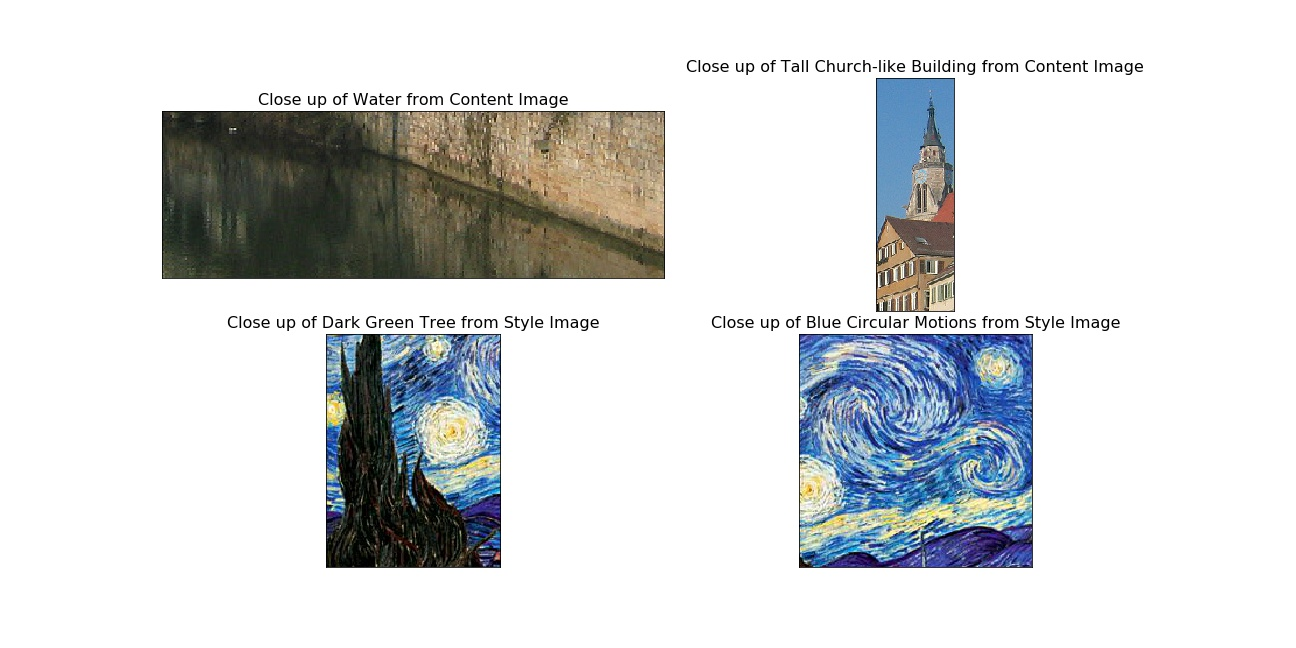
\includegraphics[width=160mm, scale = 1]{explorevisualization.jpg}
  \caption{Close-up looks at the important qualities of the content and style images. The first two are from the content image, and second two are from the style image.}
  \label{fig:explore}
\end{figure}
Some important noticeable qualities of the content image are that it is a sequence of connected houses, with a church-like building sticking out in the background (second image in Figure \ref{fig:explore}). Also, these houses are right next to a body of water (First image of Figure \ref{fig:explore}), with a tree sticking out on the left side of the image. These details of the content image are important to note because they are fundamental details, and should be expected to appear clearly in the output image. The style image (Starry Night), has some important details as well, although since it is the style of the image that matters, the objects in the image are not necessarily the fundamental details. Rather, some important details to note about this style image - that might appear in the output image - are the circular motions in the image, the different shades of blue crayon-like colouring, along with the yellow spots. the circular motins and the blue crayon-like color can be seen more clearly in the fourth image in Figure \ref{fig:explore}). Also, the dark green tree-like object on the left side of the image is an important feature because of the different color appearing on the left side only (the fact that it looks like a separate object does not matter so much, since the style of the image is of more concern than the objects themselves). Finally, the third image in Figure \ref{fig:explore} displays this dark green tree-like object clearly, and also shows an example of one of the yellow stars right next to it. In general, all of the images in Figure \ref{fig:explore} should appear somewhat clearly in the final result, since they do in Figure 2C in \cite{Neural}.


\subsection{Algorithms and Techniques}
This project uses the VGG19 network, since it was used in \cite{Neural, Image}. Since a pre-trained network is used, there is no training of the inputs, as it was not done in \cite{Neural, Image}, it takes time, and it sort of defeats the purpose of using a pre-trained network. The initial/input image is the white-noise image, and it will slowly morph into the final result, to be seen later (Figure \ref{fig:Solution}). To set up the loss function, the first step is to get the content loss function. As explained above, to get the content loss function, intermediate layer feature maps will be used iteratively to get the difference between these feature maps and the white noise feature maps, and then they will be squared and summed up. The style loss function will be obtained the same way except by using Gram matrices instead of feature maps (Gram matrices are matrices whose elements are inner/dot products of the vectorized feature maps of a given layer). The intermediate layers used will be the same ones as in \cite{Neural} (and will be accessed via eager execution in Python). Finally, the loss function will be a linear combination of the two different loss function, with coefficients that can be changed to get optimal results (some coefficient ratios are given in \cite{Neural, Image}). Since the loss function is a linear combination, both loss functions will be minimized at the same time, so the weights $\alpha$ and $\beta$ from the above equation will play an important role in getting the best model.

Gradient descent is used to minimize the loss function. The different types of gradient descent optimization functions were explored, and the Adadelta Optimizer was the optimizer that had been used. The Adadelta Optimizer is just an extension of the Adagrad Optimizer, which is an optimizer that adapts the learning rate depending upon the parameters. The normal Gradient Descent Optimizer did not give the best performance, but the Adagrad Optimizer has a disadvantage, in that it tends to agressively decrease the learning rate. The Adadelta Optimizer seeks to fix this problem, which is why it is the chosen optimizer (especially since higher learning rates seemed to be better, so decreasing it quickly may not be great in practice). Also, none of the default parameters for the Adadelta Optimizer were used, so they were all manually changed via trial and error. \cite{Neural} describes what the gradient of the content and style loss functions look like, and that standard error back-propagation can be used to calculate the gradient (a tensorflow function will do this for us). The gradients are applied to the white-noise image, and then the white noise image is de-processed so that it can be viewed. 


\subsection{Benchmark}
The benchmark model follows from the model in the methods section of \cite{Neural} and from section 2 of \cite{Image}. As just explained, the idea is to use a pre-trained image classification network to get feature maps of both the style and content images. There will be a base input image, which will be white-noise, and it will have its own feature map. The content loss function ($Loss_{content}$) will be obtained by taking the squared difference of the feature maps, and the style image will be obtained by taking the difference between gram matrices. The loss function will be as described above, and minimized with gradient descent. The ultimate benchmark result, which will be used to compare to my solution, is Figure 2c in \cite{Neural}. This whole project is about reproducing that image, and so this project is essentially a success if and only if that image is at least somewhat reproduced. 

\section{Methodology}
\subsection{Data Preprocessing}
The first pre-processing step that has been done to the inputs is that they were fixed in dimension size, with a dimension size closer to the smaller of the two input images. So, both images were fixed to a dimension of $450x338$, so that the arrays that contain their pixel information will be of same size. The second pre-processing step was to just apply the expected VGG19 preprocessing step that is normally done in Python. This is of course done to the re-sized images, and this allows the images to be used in-tandem with the tensorflow/keras libraries. The final step is to create a white-noise image for the model to take as input. Instead of getting some white noise image from google images or any other random online source, a white noise image was made from scratch using the random function. This was done by creating a white noise generator, and it was made so that each time a white-noise image was made, it would be different (with the goal of using different white-noise images to get the same result, if given enough time). The white-noise image would be of correct dimension, meaning the same dimension ($450x338$) as the input images, so this would not need to be done in a separate step. Finally, the white-noise image would also get the pre-processing step/function as expected by the VGG19 network. Now, their are the three necessary inputs, the content image, style image, and a white-noise image, all as arrays containing pixel information.

\subsection{Implementation}
When doing this project, the first thing that was done was testing it out using strictly the code from \cite{Github}. Essentially the only difference from \cite{Github} and my intended project was that \cite{Github} used the content image as the input image, and this seemed to significantly decrease run time. So I modified the goal of the project, where I borrowed a lot of code from \cite{Github}, but made some changes. The goal was now too replicate Figure 2C in \cite{Neural} in a timely manner (rather than just replicate it), with a white-noise image as the initial/input image, as was done in \cite{Neural, Image}. So the  most notable and important changes were that the input image was changed from the content image to my own generated white-noise image, and that the optimizer had changed with custom parameters (of course this problem may not have occurred given a GPU-powered computer, but no such computer was available).

So, essentially the first step was the pre-processing of the data. Then, with the content and style weights defined, the VGG19 pre-trained network is loaded and the intermediate content and style layers from \cite{Neural, Image} are called on as well (using eager execution) to get the necessary information to calculate the content and style losses. The content loss is just the euclidean distance between the feature representations  of the content image and the white-noise image, which is then squared and summed together. Now, a gram matrix takes elements as inner products of feature vectors of a given layer, and the style loss is calculated the same way as the content image, except it is a difference between theses gram matrices of the white-noise image and the style image. Next is the optimizer, and here it is the Adadelta Optimizer with hyper-parameter values: learning rate$= 8$, $\rho = 0.95$, and $\epsilon = 10^{-1}$. Using this optimizer, the gradients will be applied to the white-noise image and the loss function will be calculated. This will be done for (usually) 1000 iterations, and in each iteration, applying the gradients to the white-noise image will update it to make it look more like the intended solution, and the loss function will become the new loss function if it was better than the previous loss function value (the initial loss function value is set to negative infinity). Note that 1000 iterations took about 5 hours to run on my available computer, and this is why this project was modified (and was challenging). 

\subsection{Refinement}
The best solution is Figure \ref{fig:Solution}. Arriving at this solution involved a lot of trial and error with adjusting the parameters and hyper-parameters, for a few different optimization functions. First, the normal gradient descent was used, with various learning rates, ranging from $0.2-6$, and even $8$. Higher learning rates did not give any improvement in the loss function, and so it remained at negative infinity, and in fact, this was the case for lower learning rates. The normal/standard Gradient Descent optimizer had some success in improving the loss function with smaller learning rates, but its performance was so poor even with 1000 iterations, that I discarded it in the very beginning. The next optimizer that I tried was the Adam Optimizer function, which \cite{Github} used as well. I started with their hyper-parameter values, and tried - via trial and error - to get improved loss function values faster. After 1000 iterations, the Adam Optimizer function gave images that were starting to look like \ref{fig:Solution}, but it was not very impressive given that 1000 iterations takes roughly 5 hours. Other optimization functions were attempted after this, but none of them gave results worth mentioning, until the final two optimizers were attempted. 
\begin{figure}
\centering
  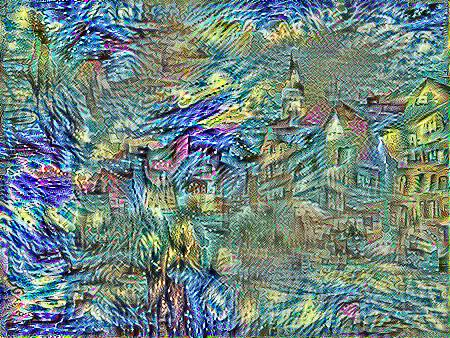
\includegraphics[width=100mm, scale = 0.5]{solution5.jpg}
  \caption{The final/best solution. Iterations: $2600$, content weight: $10^3$, style weight: $10^{-3}$}
  \label{fig:Solution}
\end{figure}

The last two optimizers were the momentum optimizer and the Adadelta Optimizer. The momentum optimizer had had only two hyper-parameters, the learning rate and momentum, and seemed to give better/faster results (still using 1000 iterations) with a learning rate of about $1$, and with a momentum value of around 0.9. This optimizer actually gave some of the better results, but the Adadelta Optimizer seemed to give slightly better results. Some intermediate results with the Adadelta Optimizer are presented in \ref{fig:IntermediateSolutions}. The default $\epsilon$ value is $10^{-8}$, and did not seem to make any significant changes to the initial white-noise image. As I attempted higher and higher $\epsilon$ values, results got better and better, until I tried $\epsilon = 1$, which seemed to be give results that were not as good as the results when $\epsilon = 10^{-1}$ or $\epsilon = 10^{-2}$. Trying $\epsilon = 2$ justified this, and this is what lead to the decision of choosing $\epsilon = 10^{-1}$. Similarly, $\rho$ values seemed to give worse results as it decreased from $0.9$, and also as it increased from $\rho = 0.99$, so $\rho = 0.95$ was chosen to be a happy medium. Finally, the learning rate was experimented with a lot, with values close to $0$, and upwards to $10$, and a value of $8$ was ultimately chosen, as it seemed produce the best/fastest result (these decision were largely decided by looking at the resulting image and comparing them, for instance, Figure \ref{fig:IntermediateSolutions} shows that when using a learning rate of 5 - even with more iterations - it seems like a learning rate of 8 is better). As such, the final solution is \ref{fig:Solution}, which was run for 2600 iterations just to give it more chances at resembling Figure \ref{fig:solution}.
\begin{figure}[h!]
  \centering
  \begin{subfigure}[b]{0.35\linewidth}
    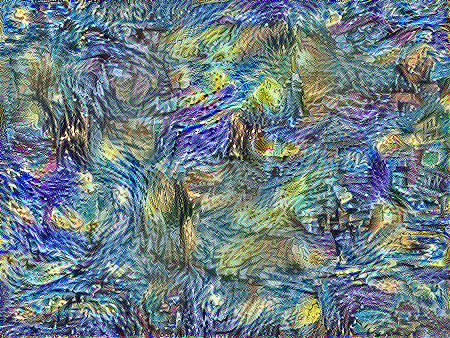
\includegraphics[width=\linewidth]{solution.jpg}
    \caption{Iterations: $2200$, content weight: $10^3$, style weight: $10^{-2}$, Learning Rate: 5, $\rho$: 0.82, $\epsilon$: $10^{-1}$}
  \end{subfigure}
  \begin{subfigure}[b]{0.35\linewidth}
    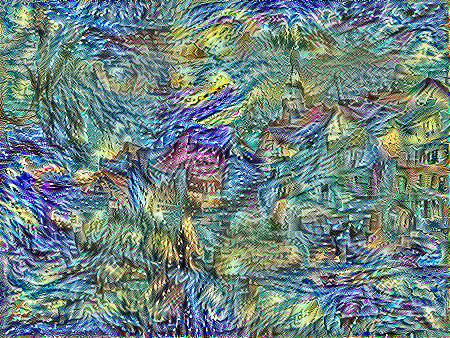
\includegraphics[width=\linewidth]{solution2.jpg}
    \caption{Iterations: $1200$, content weight: $10^4$, style weight: $10^{-2}$, Learning Rate: 8, $\rho$: 0.9, $\epsilon$: $10^{-1}$}
  \end{subfigure}
  \caption{Attempted/Intermediate solutions with the Adadelta optimizer}
  \label{fig:IntermediateSolutions}
\end{figure}




\section{Results}
\subsection{Model Evaluation and Validation}
Thus, the final model is a VGG19 pre-trained network that uses a loss function and the Adadelta optimizer to get an image aimed to look like Figure 2c in \cite{Neural}. This model is as follows from \cite{Neural, Image}, however the $\alpha$ and $\beta$ values are not quite what I would expect. Since this project's goal was to recreate an image from \cite{Neural} as closely as possible - hence why using a white-noise image was insisted upon - I would have expected the $\alpha/\beta$ ratio to be the same as \cite{Neural}. This means that I expected the final solution would have resulted in a ratio of $\alpha/\beta = 10^{-3}$, but in Figure \ref{fig:Solution}, $\alpha/\beta = 10^6$. Even \cite{Github} had $\alpha/\beta = 10^5$, so this is not entirely in line with the expected solution, as the ratio is of a large magnitude higher than expected. 

Arguably it is also expected that the model would work with any white noise image, and given the chosen optimization function (Adadelta) with its hyper-parameters as in Figure \ref{fig:Solution}, it should take a similar amount of time. This has not been tested thoroughly, although there was a mistake through the testing process where a new white noise image was created and replaced with an older one, which was meant to be used throughout the entire project. This mistake actually seemed to cause the solution to not give the same results when testing the momentum optimizer function as with the older white-noise image, and an example can be seen in Figure \ref{fig:SolutionM} (unfortunately, no previous data was saved from the older white-noise image).
\begin{figure}
\centering
  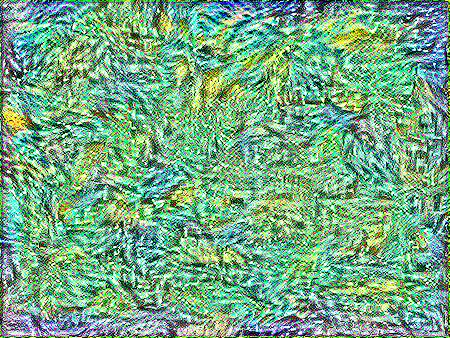
\includegraphics[width=100mm, scale = 0.5]{solution4.jpg}
  \caption{Momentum Optimizer solution with second white-noise image as input. Iterations: $1000$, Content Weight: $10^3$, Style Weight: $10^{-3}$, Learning Rate: $1$, Momentum: $0.9$}
  \label{fig:SolutionM}
\end{figure}
That being said, no apparent change was present with the Adadelta optimizer. This leads to the belief that the Adadelta optimizer allows this solution to be able to handle small changes in parameters or images (so even if the content or style images were replaced with slightly blurry versions, no noticeable difference would be visible). This would still need to be tested though (given more time, or a more powerful computer), since Figure \ref{fig:Solution} still only somewhat resembles Figure 2C in \cite{Neural}. A second run of the final solution in Figure \ref{fig:Solution} was completed with 3000 iterations, and the result is in Figure \ref{fig:Solution2}. This result is quite similar, and while two runs or data points is never enough to make any significant conclusions, it at least hints at the fact that this model is a consistent model. 

\begin{figure}
\centering
  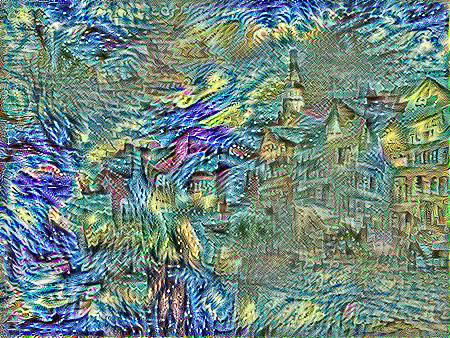
\includegraphics[width=100mm, scale = 0.5]{solution3.jpg}
  \caption{A second run of the final/best solution . Iterations: $3000$, content weight: $10^3$, style weight: $10^{-3}$}
  \label{fig:Solution2}
\end{figure}

\subsection{Justification}
The results obtained are not stronger than the benchmark or reference solution. The methods and algorithms are all the same as the benchmark solution, which comes from \cite{Neural}, but the parameters are not the same, as previously discussed. Also, a more apparent difference is that the final solution in Figure \ref{fig:Solution} is by no means identical to Figure 2c in \cite{Neural}. The solution in Figure \ref{fig:Solution} was obtained by running the program for $2600$ iterations, which took about 10 hours to complete, so clearly this program is not the optimal solution. From this alone, it is obvious that the problem has not been solved. 

Still, how well the model works can be evaluated. In terms of visual cues, when looking at Figure \ref{fig:Solution}, you can see visual aspects that are present in the intended solution in Figure 2C in \cite{Neural}. The first visual aspect to note is that the houses are visible and clearly defined, but they are still rather blurry and the colors are rather all over the place, when each house should have been one consistent color (which is actually somewhat true for the houses on the right). Another visual aspect is that the blue circular motions from the style image are appearing more so on the left side of the image, but not so much on the right, but they are still not well defined and rather blurry. The water from the content image is not clear at all, and neither are any yellow stars from the style image. These visual aspects show how far the solution is to the intended/benchmark solution, but also that it is getting closer (and possibly just needs more iterations). 

Finally, something else to compare is the loss function. Neither the extreme case of having an identical solution image to Figure 2C in \cite{Neural} with a large loss function, or the opposite extreme case, occurs in Figure \ref{fig:Solution}, so the model is at least not giving unusually/extremely poor results. The loss function value from the first iteration from Figure \ref{fig:Solution} was $143193984.0$, and the final loss function value was $1663123.5$, so the loss function's order of magnitude decreased by $10^2$. This is a good sign because the driving force of the algorithm was a decreasing loss function, and the algorithm in theory would not work without this. Figure \ref{fig:Solution2} had a final loss function value of $1020123.1$. If the model were to be rated, one way to rate it would be to take a percentage rating as the ratio of the best loss function values over the worst loss function value. Since there are only two here, the rating for this model would be $1020123.1 \div 1663123.5 = 61.3\%$. Figure \ref{fig:Solution} and Figure \ref{fig:Solution2} look quite similar, so I would have expected a higher percentage, but overall $61.3\%$ seems fair since neither Figure \ref{fig:Solution} nor Figure \ref{fig:Solution2} are identical to Figure 2C in \cite{Neural}, but the two images seem consistent with each other. Thus, the problem of this project has not been solved very well (or at all, but it seems like it is getting there).

\section{Conclusion}
\subsection{Free-Form Visualization}
An important quality of this project is showing that the idea of style transfer is clear, and the general ideas behind it work. In Figure \ref{fig:Visual}, you can see the process of the implementation, and the slow changes that occur. The first image in Figure \ref{fig:Visual} is just the white-noise image, as this is the initial image. The second image comes from the fourteenth iteration and essentially still looks like white-noise, but if you look closely, you can see slight changes in the image, and circular motions in the image start to form (circular motions come from the style image, as discussed in the Exploratory Visualization section). In the third image, these circular motions become more apparent, and even more so in the fourth image. Also, in the fourth image, if you look closely enough, the houses from the content image start to take form, and are much more defined in the fifth image. Finally, in the sixth and final image, which is also the solution from Figure \ref{fig:Solution}, the houses from the content image and the circular motions from the style image are clearly present. This is to show that as the loss function values decrease, the image does clearly start to look more like both the style and content images. Thus, from this project alone, one can conclude that the idea of style transfer is reasonable and this method is a practical one.
\begin{figure}
  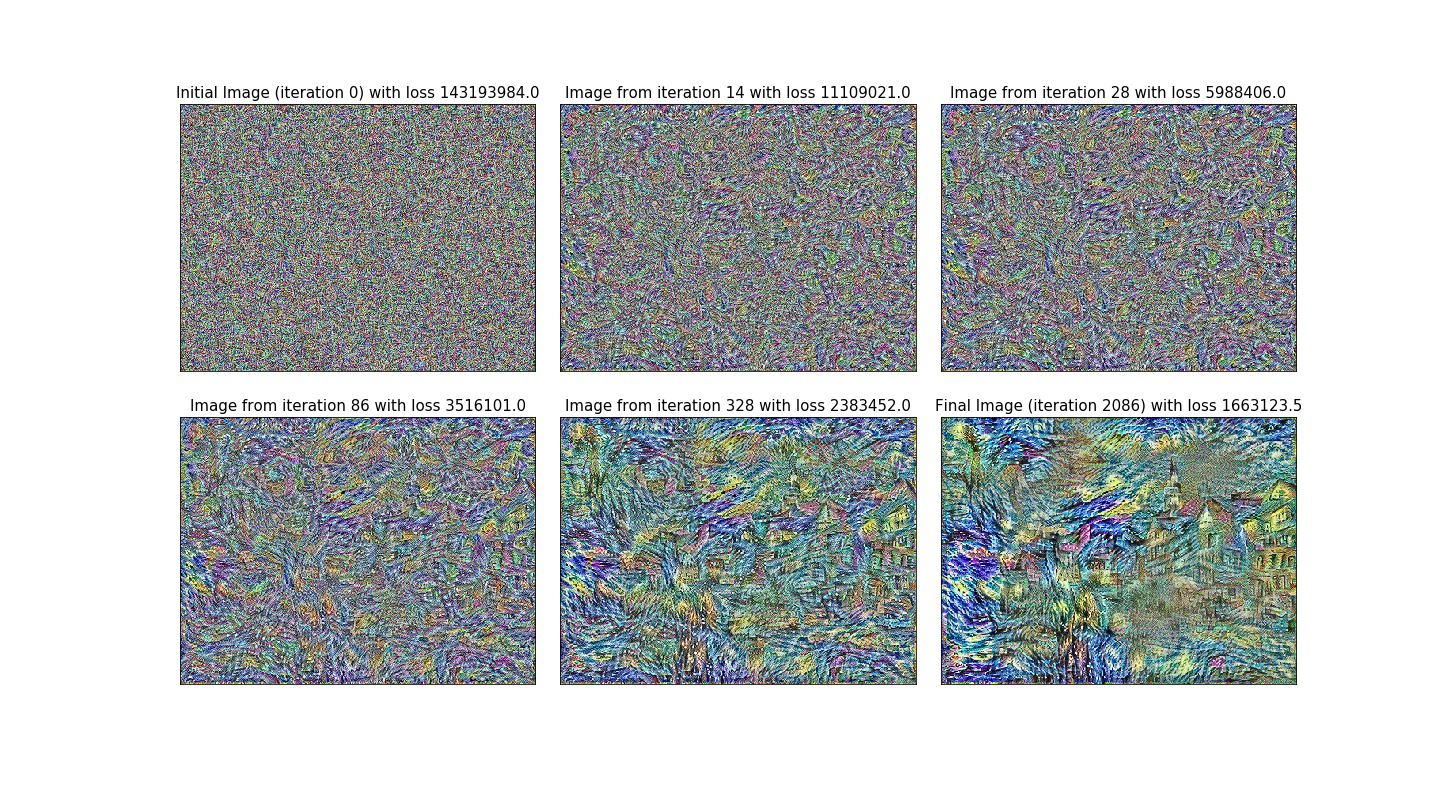
\includegraphics[width=150mm]{visualization.jpg}
  \caption{The slow process of the final/best solution visualized with the first image, four intermediate images, and the final image.}
  \label{fig:Visual}
\end{figure}

\subsection{Reflection}
Essentially, this project amounted to a lot of parameter and hyper-parameter fine tuning, mostly by the means of trial and error, but also by some intuitive analysis regarding which optimization function to use (\cite{GD} was a useful resource in this regard). It started with creating a white noise image, and pre-processing it along with the content and style images. Then, using the content and style loss functions from \cite{Github} (which used information from feature maps from the same intermediate layers as \cite{Neural}), the total loss function was minimized with an optimization function. Since minimizing the loss function was the ultimate goal, the optimization function was arguably the most important part when trying to obtain a result similar to that of Figure 2C in \cite{Neural}, hence why so much fine tuning was done during the process of getting the solution in Figure \ref{fig:Solution}. By far the most difficult problem encountered during this project was dealing with the long run time. It is clear from Figure \ref{fig:Visual} that at least $1000$ iterations is necessary for the result to at least somewhat resemble either the content or style images, but it takes roughly five hours to do this, and to do it over and over again while continuously trying new parameter and hyper-parameter values is just not practical. In the beginning, since a pre-trained network was going to be used, I thought perhaps the runtime would not be absurdly long, but given that it is, it is clear that the final solution is not to be used in a general setting, unless perhaps a more powerful computer is used. That being said, it was interesting to see how the white-noise image slowly changed into the final result, and how - usually - the circular motions from the style image always seemed to appear before the content images houses. It would also be interesting to see how well this would work with other content and style image combinations, but again, this project is just not practical with a such a long runtime.

\subsection{Improvement}
One obvious improvements to this project would be to get a much more powerful computer to handle the image processing in this project. The average runtime for each result was about five hours, so even decreasing that to one hour would make this project much more viable since many more iterations seem to be necessary. Another improvement, or something to consider doing for next time, would be to implement some function that would save the result of each final result, along with the parameters, hyper-parameters, and loss function values. This is because in the beginning it just did not seem necessary since I was just testing things out, with the expectation that soon I would produce an image identical to Figure 2c in \cite{Neural}, but slowly time decreased, and it became apparent that Figure 2c in \cite{Neural} was unlikely to be reproduced, and that those previous results may have been beneficial for comparisons. 

Some other things to try would be different optimization functions. Some others were attempted, but only for a few runs with much less iterations since time was low, and they ended up being discarded quickly. These other optimizations were just slight variations of the ones already mentioned, like the Adagrad Optimizer, and even the RMSprop optimizer. There are also other optimizers that might be worth trying that I am unfamiliar with, like the Proximal Adagrad Optimizer, as well the the Proximal Gradient Descent Optimizer. Another thing to try would be to use different intermediate layers than presented in \cite{Image}, but exactly how these would affect the result would need to be explored, otherwise it would be another long trial and error process. If someone else were to repeat this project, and use Figure \ref{fig:Solution} as a benchmark solution, it is likely that a better solution would be found, but perhaps with these other optimizers mentioned or with other intermediate layers, there exists a solution that would make it much more practical on a computer that is comparatively just as powerful/limited as mine.




\newpage

\bibliographystyle{unsrt}
\addcontentsline{toc}{section}{Bibliography}
\bibliography{Bibliographyproposal}

\end{document}